\documentclass{beamer}
\usepackage[utf8]{inputenc}
  
\usetheme{Madrid}
\usecolortheme{default}
\usepackage{amsmath,amssymb,amsfonts,amsthm}
\usepackage{txfonts}
\usepackage{tkz-euclide}
\usepackage{listings}
\usepackage{adjustbox}
\usepackage{array}
\usepackage{tabularx}
\usepackage{gvv}
\usepackage{lmodern}
\usepackage{circuitikz}
\usepackage{tikz}
\usepackage{graphicx}
\usepackage[T1]{fontenc}
\UseRawInputEncoding

\setbeamertemplate{page number in head/foot}[totalframenumber]

\usepackage{tcolorbox}
\tcbuselibrary{minted,breakable,xparse,skins}



\definecolor{bg}{gray}{0.95}
\DeclareTCBListing{mintedbox}{O{}m!O{}}{%
  breakable=true,
  listing engine=minted,
  listing only,
  minted language=#2,
  minted style=default,
  minted options={%
    linenos,
    gobble=0,
    breaklines=true,
    breakafter=,,
    fontsize=\small,
    numbersep=8pt,
    #1},
  boxsep=0pt,
  left skip=0pt,
  right skip=0pt,
  left=25pt,
  right=0pt,
  top=3pt,
  bottom=3pt,
  arc=5pt,
  leftrule=0pt,
  rightrule=0pt,
  bottomrule=2pt,
  toprule=2pt,
  colback=bg,
  colframe=orange!70,
  enhanced,
  overlay={%
    \begin{tcbclipinterior}
    \fill[orange!20!white] (frame.south west) rectangle ([xshift=20pt]frame.north west);
    \end{tcbclipinterior}},
  #3,
}
\lstset{
    language=C,
    basicstyle=\ttfamily\small,
    keywordstyle=\color{blue},
    stringstyle=\color{orange},
    commentstyle=\color{green!60!black},
    numbers=left,
    numberstyle=\tiny\color{gray},
    breaklines=true,
    showstringspaces=false,
}



\title 
{MatGeo Assignment 4.4.3}

\author
{AI25BTECH11007}
\begin{document}

\frame{\titlepage}
\begin{frame}{Question}
Equation of the line passing through the origin and making $30^\circ$
, $60^\circ$, and $90^\circ$ with the $X, Y, Z$ axes respectively is.
\end{frame}

\begin{frame}{Solution}
    The equation of a line passing through the origin and making angles 
$\alpha, \beta, \gamma$ with the $X, Y, Z$ axes respectively is given by
\[
\frac{x}{\cos \alpha} = \frac{y}{\cos \beta} = \frac{z}{\cos \gamma}.
\]
Here, $\alpha = 30^\circ, \beta = 60^\circ, \gamma = 90^\circ$.\\

Direction Cosines,
\[
\cos 30^\circ = \frac{\sqrt{3}}{2}, \quad 
\cos 60^\circ = \frac{1}{2}, \quad 
\cos 90^\circ = 0.
\]

\[
\frac{x}{\frac{\sqrt{3}}{2}} = \frac{y}{\frac{1}{2}} = \frac{z}{0}.
\]


Final equation of the line ,
\[
y = \frac{x}{\sqrt{3}}, \quad z = 0.
\]
\end{frame}

\begin{frame}{Plot}
    \begin{figure}[H]
    \centering
    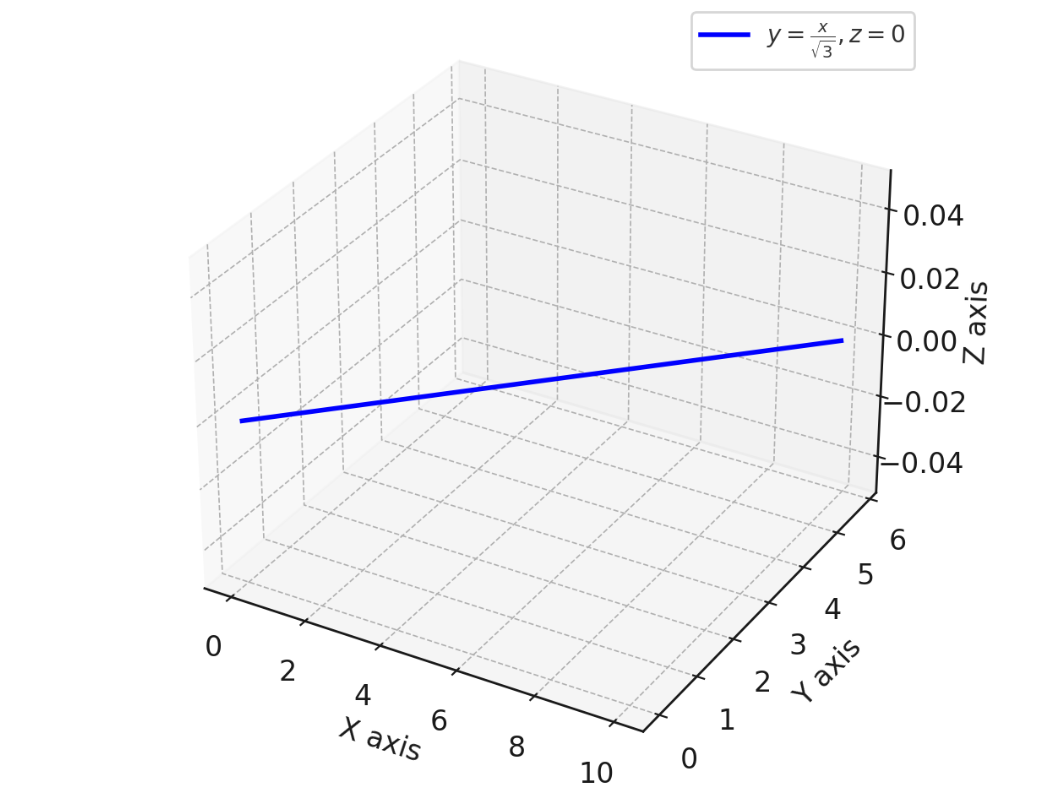
\includegraphics[width=0.85\linewidth]{figs/image.png}
    \caption{Plot}
    \label{fig:placeholder}
\end{figure}
\end{frame} 

\begin{frame}[fragile]{C code}
\begin{lstlisting}[language = c]
#include <stdio.h>
#include <math.h>

int main() {
    // Angles in degrees
    double alpha = 30.0, beta = 60.0, gamma = 90.0;

    // Direction cosines
    double lx = cos(alpha * M_PI / 180.0);
    double ly = cos(beta * M_PI / 180.0);
    double lz = cos(gamma * M_PI / 180.0);

    printf("Direction cosines:\n");
    printf("cos(30) = %.3f\n", lx);
    printf("cos(60) = %.3f\n", ly);
    printf("cos(90) = %.3f\n", lz);
\end{lstlisting}
\end{frame}

\begin{frame}[fragile]{C code}
\begin{lstlisting}[language = c]
// Equation of line through origin: (x/lx) = (y/ly) = (z/lz)
printf("\nEquation of line:\n");
printf("y = x / sqrt(3),  z = 0\n");

    // Verify with some values of x
    printf("\nSample points on the line:\n");
    for (int x = 0; x <= 6; x += 2) {
        double y = x / sqrt(3);
        double z = 0;
        printf("(%.2f, %.2f, %.2f)\n", (double)x, y, z);
    }

    return 0;
}
\end{lstlisting}  
\end{frame}

\begin{frame}[fragile]{Python Code}
 \begin{lstlisting}
     import numpy as np
import matplotlib.pyplot as plt

# Angles in degrees
alpha, beta, gamma = 30, 60, 90

# Direction cosines
lx = np.cos(np.radians(alpha))
ly = np.cos(np.radians(beta))
lz = np.cos(np.radians(gamma))

print("Direction cosines:")
print(f"cos(30°) = {lx:.3f}")
print(f"cos(60°) = {ly:.3f}")
print(f"cos(90°) = {lz:.3f}")

print("\nEquation of the line:")
print("y = x / sqrt(3),  z = 0")
\end{lstlisting}   
\end{frame}

\begin{frame}[fragile]{Python Code}
 \begin{lstlisting}
x_vals = np.linspace(0, 10, 6)
y_vals = x_vals / np.sqrt(3)
z_vals = np.zeros_like(x_vals)
print("\nSample points on the line:")
for x, y, z in zip(x_vals, y_vals, z_vals):
    print(f"({x:.2f}, {y:.2f}, {z:.2f})")
# Plot the line in 3D
fig = plt.figure(figsize=(8,6))
ax = fig.add_subplot(111, projection='3d')
ax.plot(x_vals, y_vals, z_vals, label=r'$y = \frac{x}{\sqrt{3}}, z=0$', color='blue', linewidth=2)

ax.set_xlabel('X axis')
ax.set_ylabel('Y axis')
ax.set_zlabel('Z axis')
ax.set_title('Line through origin making 30°, 60°, 90° with X, Y, Z axes')
ax.legend()
plt.show()

\end{lstlisting}   
\end{frame}
\end{document}